\documentclass[tikz,border=3pt]{standalone}
\usepackage[utf8]{inputenc}
\usepackage[T1]{fontenc}
\usepackage{lmodern}
\renewcommand{\familydefault}{\sfdefault}
\usepackage{sansmath}\sansmath
\usepackage{chemfig}
\usepackage{pgfplots}\pgfplotsset{compat=1.18,/pgf/number format/use comma,/pgf/number format/1000 sep={.}}
\usetikzlibrary{arrows.meta,calc,positioning,decorations.pathmorphing,patterns}
% paleta del sitio
\definecolor{nar}{HTML}{E8680C}\definecolor{narc}{HTML}{FFB35C}\definecolor{hielo}{HTML}{FFF3E8}
\definecolor{tinta}{HTML}{1D1D1F}\definecolor{gris}{HTML}{6E6E73}\definecolor{lila}{HTML}{7C5CF0}
\definecolor{azul}{HTML}{2F6FD6}\definecolor{menta}{HTML}{17A673}\definecolor{coral}{HTML}{E8342A}
\tikzset{cel/.style={draw=gris,fill=hielo,line width=0.9pt},nuc/.style={draw=gris!70,line width=0.6pt},
fib/.style={gris!55,line width=0.35pt},eti/.style={font=\footnotesize,text=tinta,align=center},
num/.style={circle,draw=nar,fill=white,text=nar,font=\small\bfseries,inner sep=1.2pt,minimum size=13pt},
fl/.style={-{Stealth[length=2.6mm]},gris,line width=0.9pt}}
\begin{document}
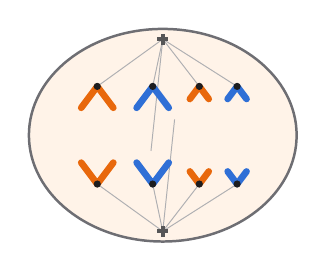
\begin{tikzpicture}[font=\small]
\draw[cel] (0,0) ellipse (1.7 and 1.35);
\draw[fib] (0,1.22)--(-0.832,0.62);
\draw[fib] (0,-1.22)--(-0.832,-0.62);
\draw[fib] (0,1.22)--(-0.128,0.62);
\draw[fib] (0,-1.22)--(-0.128,-0.62);
\draw[fib] (0,1.22)--(0.464,0.62);
\draw[fib] (0,-1.22)--(0.464,-0.62);
\draw[fib] (0,1.22)--(0.944,0.62);
\draw[fib] (0,-1.22)--(0.944,-0.62);
\draw[fib] (0,1.22)--(-0.15,-0.2);
\draw[fib] (0,-1.22)--(0.15,0.2);
\begin{scope}[shift={(-0.832,0.62)},rotate=0]\draw[nar,line width=2.4pt,line cap=round,line join=round] (-0.204,-0.272)--(0,0)--(0.204,-0.272);\end{scope}
\fill[tinta] (-0.832,0.62) circle (1.3pt);
\begin{scope}[shift={(-0.832,-0.62)},rotate=180]\draw[nar,line width=2.4pt,line cap=round,line join=round] (-0.204,-0.272)--(0,0)--(0.204,-0.272);\end{scope}
\fill[tinta] (-0.832,-0.62) circle (1.3pt);
\begin{scope}[shift={(-0.128,0.62)},rotate=0]\draw[azul,line width=2.4pt,line cap=round,line join=round] (-0.204,-0.272)--(0,0)--(0.204,-0.272);\end{scope}
\fill[tinta] (-0.128,0.62) circle (1.3pt);
\begin{scope}[shift={(-0.128,-0.62)},rotate=180]\draw[azul,line width=2.4pt,line cap=round,line join=round] (-0.204,-0.272)--(0,0)--(0.204,-0.272);\end{scope}
\fill[tinta] (-0.128,-0.62) circle (1.3pt);
\begin{scope}[shift={(0.464,0.62)},rotate=0]\draw[nar,line width=2.4pt,line cap=round,line join=round] (-0.12,-0.16)--(0,0)--(0.12,-0.16);\end{scope}
\fill[tinta] (0.464,0.62) circle (1.3pt);
\begin{scope}[shift={(0.464,-0.62)},rotate=180]\draw[nar,line width=2.4pt,line cap=round,line join=round] (-0.12,-0.16)--(0,0)--(0.12,-0.16);\end{scope}
\fill[tinta] (0.464,-0.62) circle (1.3pt);
\begin{scope}[shift={(0.944,0.62)},rotate=0]\draw[azul,line width=2.4pt,line cap=round,line join=round] (-0.12,-0.16)--(0,0)--(0.12,-0.16);\end{scope}
\fill[tinta] (0.944,0.62) circle (1.3pt);
\begin{scope}[shift={(0.944,-0.62)},rotate=180]\draw[azul,line width=2.4pt,line cap=round,line join=round] (-0.12,-0.16)--(0,0)--(0.12,-0.16);\end{scope}
\fill[tinta] (0.944,-0.62) circle (1.3pt);
\fill[tinta!75] (-0.07,1.195) rectangle (0.07,1.245);\fill[tinta!75] (-0.025,1.15) rectangle (0.025,1.29);
\fill[tinta!75] (-0.07,-1.245) rectangle (0.07,-1.195);\fill[tinta!75] (-0.025,-1.29) rectangle (0.025,-1.15);
\end{tikzpicture}
\end{document}
